% Шаблон (версия от 15.02.2016) предназначен 
% для использования студентами каф. ПМиИ СамГТУ 
% при оформлении отчетов по лабораторным работам. 
% Для настройки пакета listigs использовался материал 
% статьи Михаила Конника aka virens
% <http://mydebianblog.blogspot.ru/2012/12/latex.html>
% Copyright (c) 2016 by Mikhail Saushkin (msaushkin@gmail.com) 
% All rights reserved except the rights granted by the
% Creative Commons Attribution 4.0 International Licence
% <https://creativecommons.org/licenses/by/4.0/>
% Свежая версия шаблона здесь <https://www.overleaf.com/read/sqvxbnhgxxdm>
\documentclass[14pt,a4paper,report]{ncc}
\usepackage[a4paper, mag=1000, left=2.5cm, right=1cm, top=2cm, bottom=2cm, headsep=0.7cm, footskip=1cm]{geometry}
\usepackage[utf8]{inputenc}
\usepackage[english,russian]{babel}
\usepackage{indentfirst}
\usepackage[dvipsnames]{xcolor}
\usepackage[colorlinks]{hyperref}
\usepackage{listings} 
\usepackage{caption}
\usepackage{amssymb}
\usepackage{tcolorbox}
\DeclareCaptionFont{white}{\color{white}} %% это сделает текст заголовка белым
%% код ниже нарисует серую рамочку вокруг заголовка кода.
\usepackage{color} %% это для отображения цвета в коде
\DeclareCaptionFormat{listing}{\colorbox{gray}{\parbox{\textwidth}{#1#2#3}}}
\captionsetup[lstlisting]{format=listing,labelfont=white,textfont=white}
\lstset{% Собственно настройки вида листинга
inputencoding=utf8, extendedchars=\true, keepspaces = true, % поддержка кириллицы и пробелов в комментариях
language=C++,            % выбор языка для подсветки (здесь это Pascal)
numberstyle =\tiny
basicstyle=\small\sffamily, % размер и начертание шрифта для подсветки кода
keywordstyle =\color{ForestGreen},
numbers=left,               % где поставить нумерацию строк (слева\справа)
numberstyle=\tiny,          % размер шрифта для номеров строк
stepnumber=1,               % размер шага между двумя номерами строк
numbersep=5pt,              % как далеко отстоят номера строк от подсвечиваемого кода
backgroundcolor=\color{white}, % цвет фона подсветки - используем \usepackage{color}
showspaces=false,           % показывать или нет пробелы специальными отступами
showstringspaces=false,     % показывать или нет пробелы в строках
showtabs=false,             % показывать или нет табуляцию в строках
frame=single,               % рисовать рамку вокруг кода
tabsize=2,                  % размер табуляции по умолчанию равен 2 пробелам
captionpos=t,               % позиция заголовка вверху [t] или внизу [b] 
breaklines=true,            % автоматически переносить строки (да\нет)
breakatwhitespace=false,    % переносить строки только если есть пробел
escapeinside={\%*}{*)}      % если нужно добавить комментарии в коде
}

\begin{document}
% Переоформление некоторых стандартных названий
%\renewcommand{\chaptername}{Лабораторная работа}
\def\contentsname{Содержание}

% Оформление титульного листа
\begin{titlepage}
\begin{center}
\textsc{ФГОУ ВО Уральский Федеральный Университет \\ имени первого Президента России Б.Н.Ельцина\\[5mm]
Физико-технологический институт\\[2mm]
Кафедра теоретической физики и прикладной математики}

\vfill

\textbf{ОТЧЁТ ПО ЛАБОРАТОРНОЙ РАБОТЕ №5\\[3mm]
«Разработка компьютерной программы для генерирования ячеечной перколяции на квадратной решетке со стороной L»\\[6mm]
}
\end{center}

\hfill
\begin{minipage}{.5\textwidth}
Студент:\\[2mm] 
Вялова С.А.\\
группа: ФтМ-170403 \\[5mm]

Преподаватель:\\[2mm] 
д.ф.-м.н., профессор\\
Мазуренко Владимир Владимирович\\[5mm]

Консультант:\\[2mm] 
н.с.\\
Сотников Олег Михайлович\\

\end{minipage}%
\vfill
\begin{center}
\today  \\
%\theyear\, г.
 Екатеринбург.
\end{center}
\end{titlepage}

% Содержание
\tableofcontents
\newpage
\chapter{Разработка компьютерной программы для генерирования ячеечной перколляции на квадратной решетке со стороной L}
\section{Цель работы}
Разработка компьютерной программы для генерирования ячеечной перколяции на квадратной решетке со стороной $L$; оценка значения порога перколяции $p_c$ по результатам десяти испытаний для квадратной решетки со сторонами $L=4$, $L=16$, $L=32$. Анализ динамики порога перколяции в зависимости от величины стороны решетки.
\newpage\section{Теоретическая часть}
\subsection{Перколляция}
Перколяция является удобной моделью для описания широкого класса явлений, которые принято называть критическими. Перколяционные процессы могут приводить к самоорганизации и образованию структур. Объекты, которые образуются при перколяции, называются фракталами. Два простейших типа задач формулируются путём представления среды в виде дискретной решётки. Можно выборочно случайным образом красить (открывать) узлы решётки, считая долю крашенных узлов основным независимым параметром и полагая два крашенных узла принадлежащими одному кластеру, если их можно соединить непрерывной цепочкой соседних крашенных узлов.
\

Рассмотрим квадратную сетку размером со стороной $L=3$. Случайным образом выберем три ячейки сетки и заполним их. Тогда доля заполненных ячеек будет составлять $p={N_{filled}}/N$, где $N$ - общее число ячеек в сетке.
\

Один из основных вопросов, на который пытается ответить теория перколяции, - при какой доле $p_c$ заполненных ячеек возникает цепочка, соединяющая верхнюю и нижнюю стороны сетки. Для сетки конечного размера такие цепочки - перколяционные кластеры - могут возникать при разных концентрациях. Если размер сетки $L$ устремить к бесконечности, то критическая концентрация $p_c$, называющаяся порогом перколляции, станет вполне определённой (рис. 1.1). 
\begin{figure}[!h]
\center{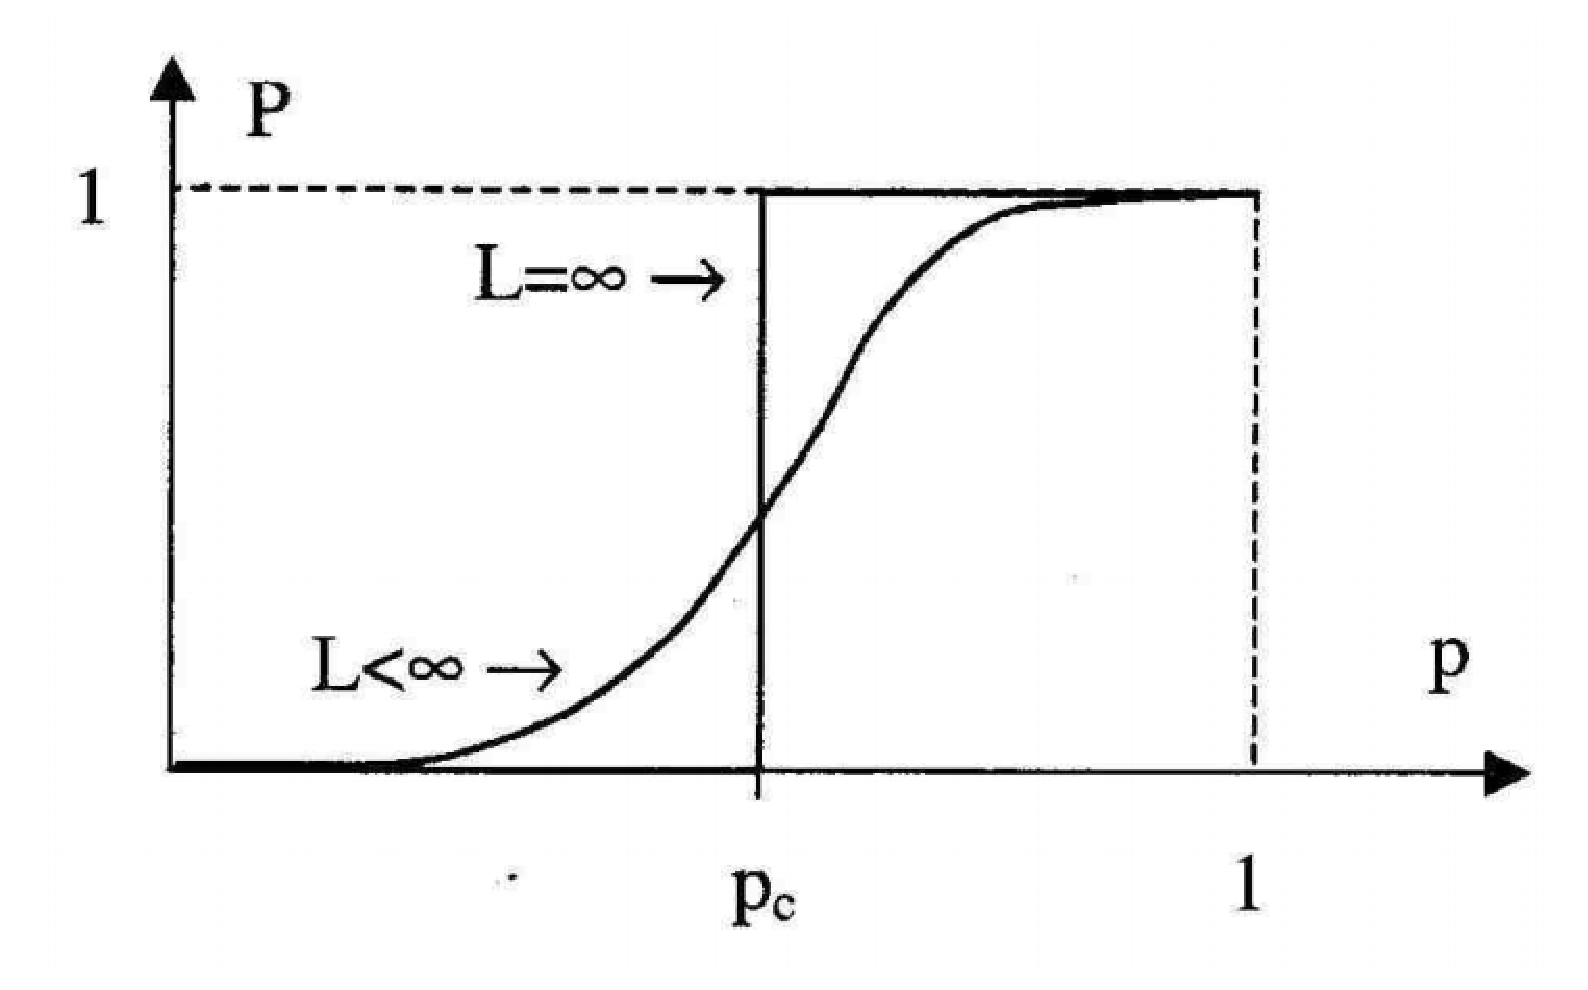
\includegraphics[width=0.6\linewidth]{ppc}}
\caption{Вероятность возникновения перколяции P в зависимости от доли заполненных узлов p. Гладкая кривая соответствует решетке конечного размера, ступенчатая - бесконечно большой решетке.}
\end{figure}

Решеточные модели в первую очередь представляют интерес с теоретической точки зрения. К настоящему времени процессы протекания на решетках изучены и поняты достаточно хорошо. С другой стороны, эти задачи имеют и практическую значимость: такой модели достаточно, чтобы описать фазовый переход парамагнетик-ферромагнетик, процес распространения эпидемии, лесного пожара. В химии теория перколляции применяется для описания процессов порлимеризации или связывания маленьких молекул в макромолекулы (гели). Кроме того, теория находит широкое применение для описания различных неупорядоченных систем в химии и физике: пористые и аморфные материалы, включая и тонкие пленки; неупорядоченные ионные проводники; галактические структуры.
\ 

Кластером в теории перколяции называется цепочка связанных объектов (например, заполненных ячеек). Перколяционным кластером называется кластер, соединяющий две противоположные стороны системы.
\


В настоящей работе будет оцениваться порог перколяции $p_c$ для решетки со стороной $L$ для случаев $L=4$, $L=16$, $L=32$. Пусть $p$ - вероятность того, что в заполненной ячейке отыщется хотя бы один перколяционный кластер. Начальное значение $p$ выбрано равным 0,2. В исходном состоянии решетка не имеет заполненых ячеек. Ячейки решетки будут заполняться последовательно исходя из следующего условия: генерируется случайное число $n$. Если $n$ меньше либо равно $p$, то ячейка заполняется, если больше - остается пустой. В заполненной решетке регистрируется наличие перколяционного кластера и фиксируется значение $p$, когда такой кластер появляется впервые. Затем значение $p$ увеличивается на 0.025, после чего последовательность действий повторяется. Для каждого значения $L$ процедура повторяется 10 раз и для каждого $L$ оценивается порог перколяции как среднее значение по десяти испытаниям.

\newpage\section{Практическая часть}
\subsection{Разработка программы}
Целью настоящей работы является разработка компьютерной программы для генерирования ячеечной перколяции на квадратной решетке со стороной $L$. Программа реализована на языке C++. Алгоритм программы реализован следующим образом: пусть квадратная решетка со стороной $L$ представляется в виде двумерного массива $L  \times L$ типа $boolean$. В начальный момент времени массив заполнен нулями. Также задаётся некоторое значение $p$, при котором маловероятно наличие соединяющего кластера. В данном случае выбрано значение $p$, равное 0.2. В цикле по строкам и столбцам массива, моделирующего решетку, генерируется случайное число n от 0 до 1, которое сравнивается с текущим значением $p$: если $n$ окажется не больше $p$, то значение элемента массива с индексом $(i,j)$ принимает значение логической единицы, то есть ячейка заполняется. При этом в отдельный файл $coordinates$ выводятся индексы заполненного элемента массива - координата заполненной ячейки. По окончании заполнения массива в этот же файл выводится значение $p$. После цикла заполнения массива значение $p$ увеличивается на 0.025, и цикл заполнения повторяется до некоторого конечного значения $p$, в данном случае выбрано 0.9. На выходе программы имеется текстовый файл с координатами всех заполненных ячеек решетки, вероятностью заполнения, который является входным файлом для программы визуализации решетки. В данном случае использован пакет $GNUplot$.
\

\subsection{Обработка результатов моделирования}
Разработанная в рамках данной работы программа запускается при помощи скрипта в коммандной оболочке $bash$. Скрипт запускает программу с заданным параметром $L$, затем GNUplot с необходимым конфигурационным файлом, определённым для каждого значения $L$, после чего просмотрщик изображений, в котором отображается полученные изображения заполненных решеток (рис. 1.2-1.7).
\ 


\begin{figure}[h!]
\begin{center}
\begin{minipage}[h!]{0.38\linewidth}
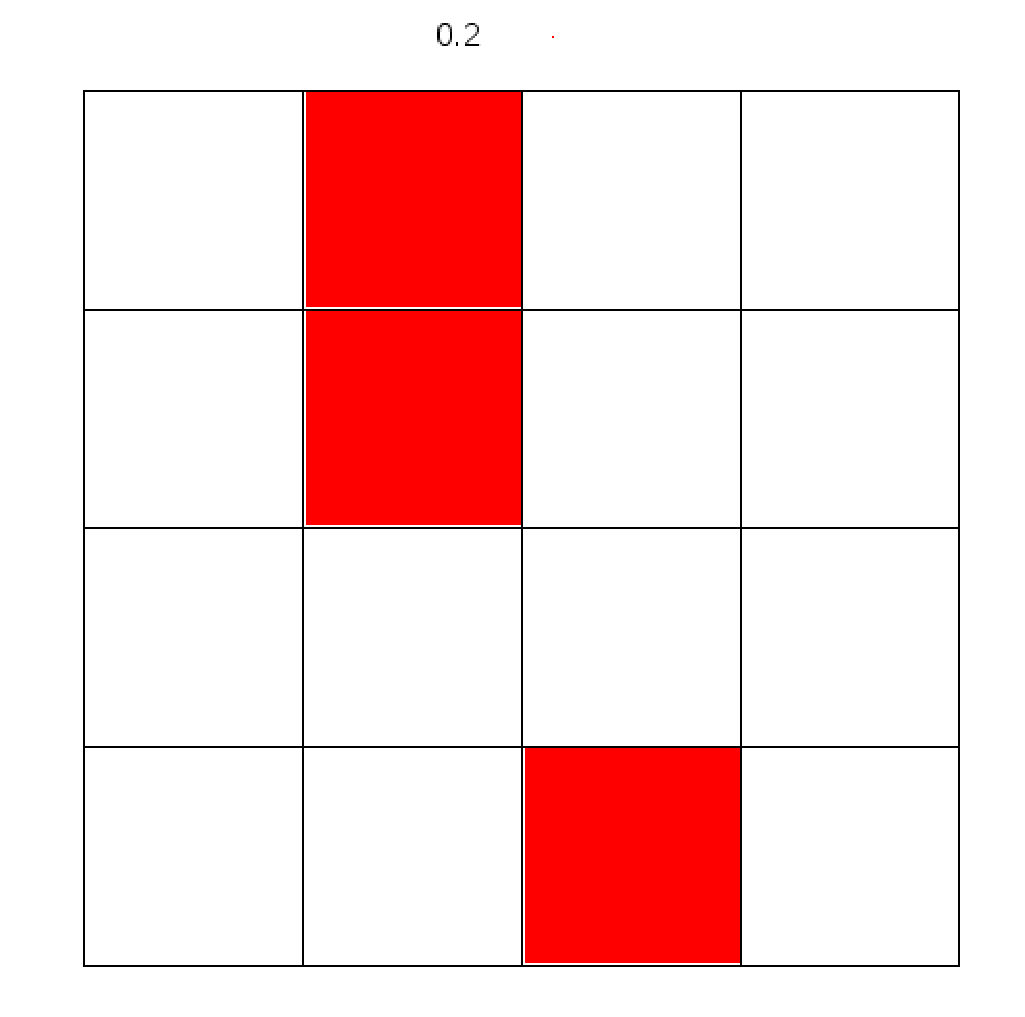
\includegraphics[width=1\linewidth]{L4_1}
\caption{Характерный вид заполненной решетки для $L=4$, в верхней части изображения отображается текущее значение $p$.} %% подпись к рисунку
\label{ris:experimoriginal} %% метка рисунка для ссылки на него
\end{minipage}
\hfill
\begin{minipage}[h!]{0.45\linewidth}
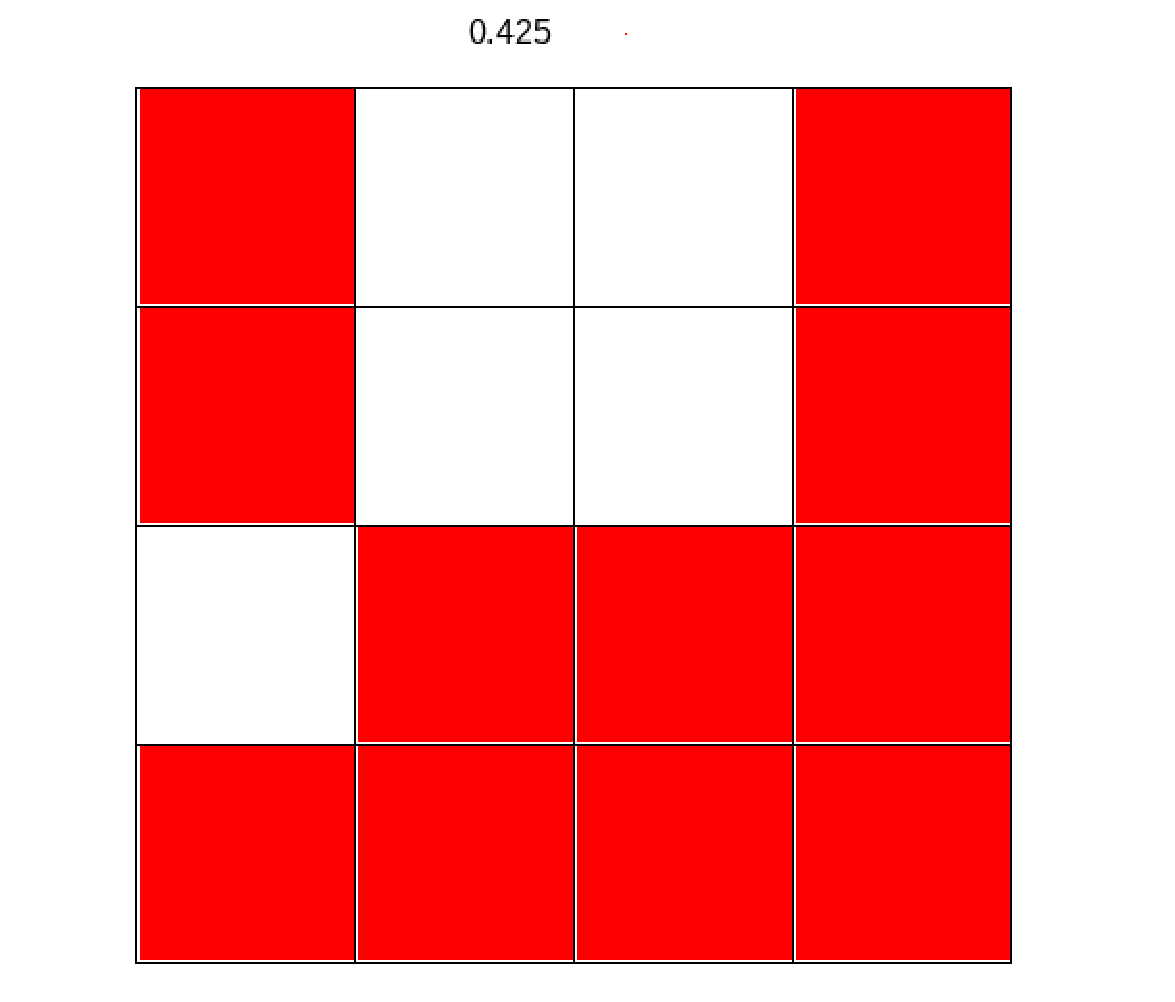
\includegraphics[width=1\linewidth]{L4_2}
\caption{Характерный вид заполненной решетки для $L=4$, в верхней части изображения отображается текущее значение $p$. В данном случае появился перколяционный кластер.}
\label{ris:experimcoded}
\end{minipage}
\end{center}
\end{figure}

\begin{figure}[h!]
\begin{center}
\begin{minipage}[h!]{0.45\linewidth}
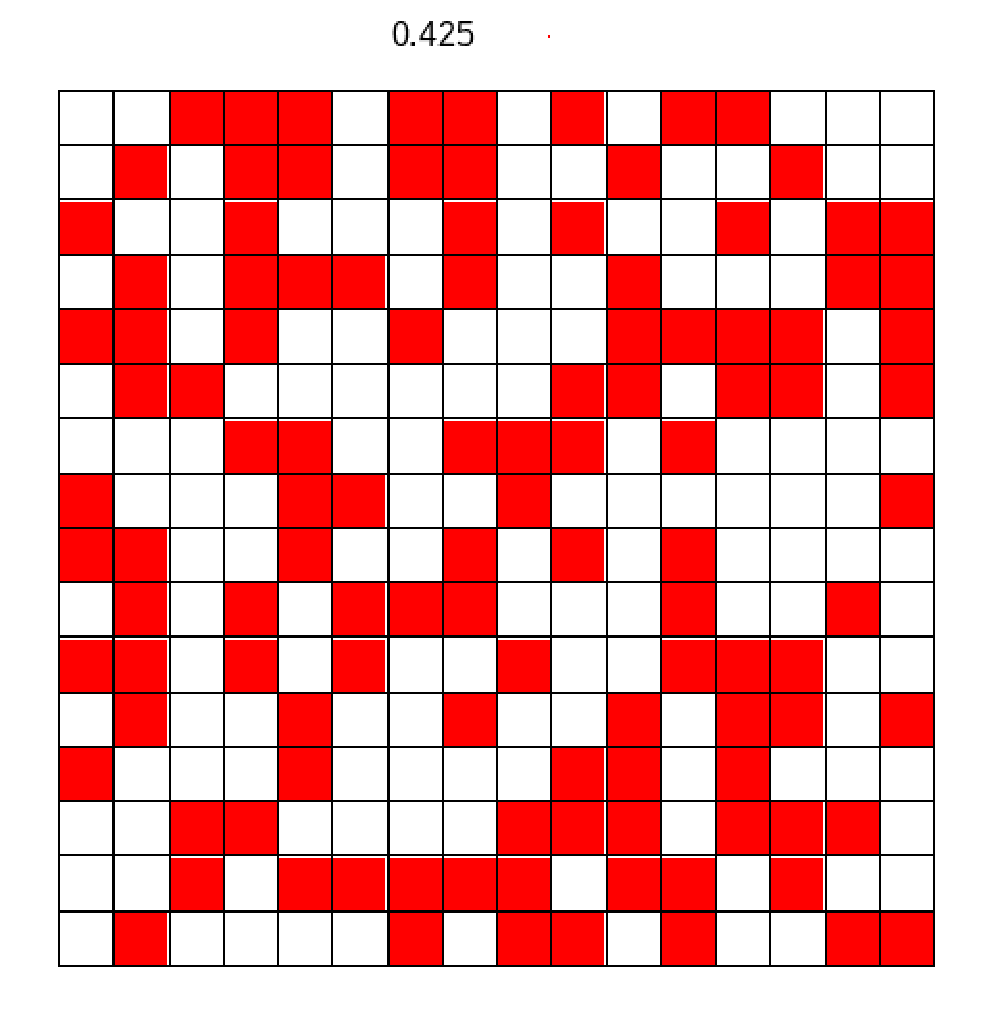
\includegraphics[width=1\linewidth]{L16_1}
\caption{Характерный вид заполненной решетки для $L=16$, в верхней части изображения отображается текущее значение $p$.} %% подпись к рисунку
\label{ris:experimoriginal} %% метка рисунка для ссылки на него
\end{minipage}
\hfill
\begin{minipage}[h!]{0.45\linewidth}
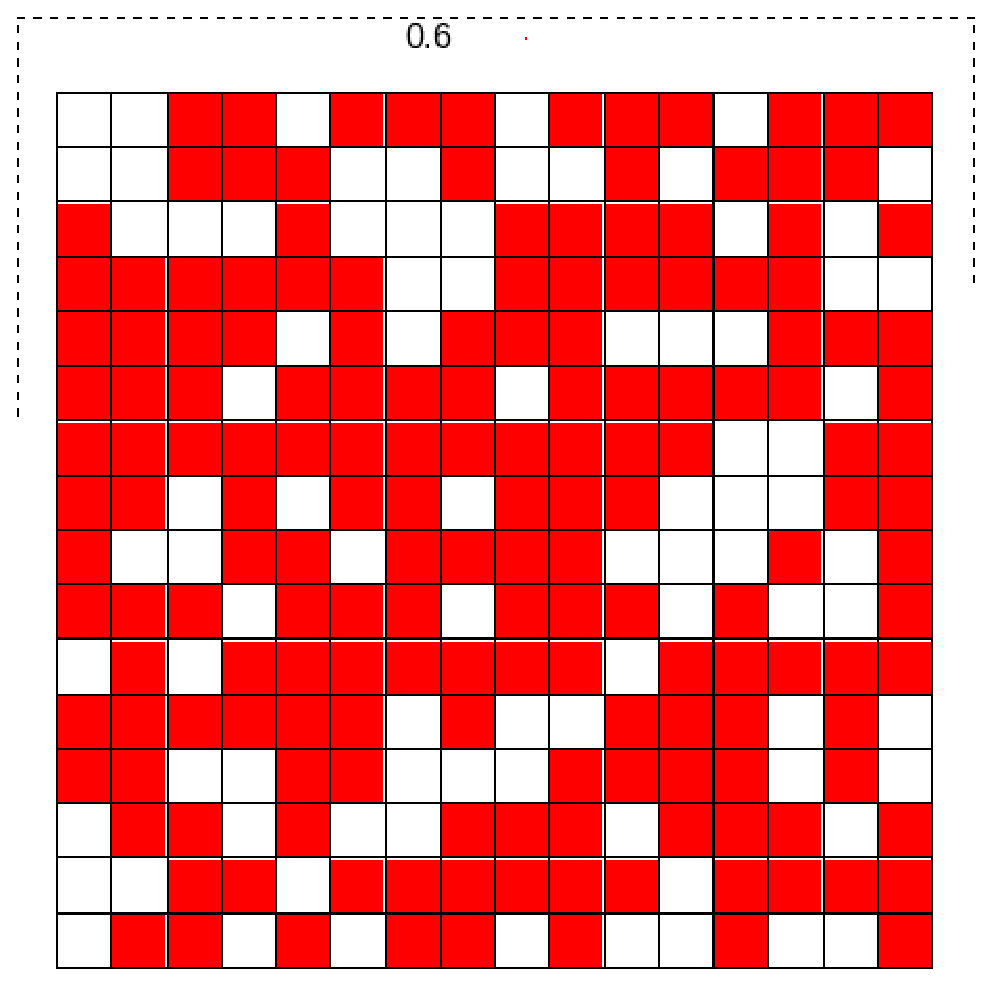
\includegraphics[width=1\linewidth]{L16_2}
\caption{Характерный вид заполненной решетки для $L=16$. В данном случае появился перколяционный кластер.}
\label{ris:experimcoded}
\end{minipage}
\end{center}
\end{figure}

\begin{figure}[h!]
\begin{center}
\begin{minipage}[h!]{0.49\linewidth}
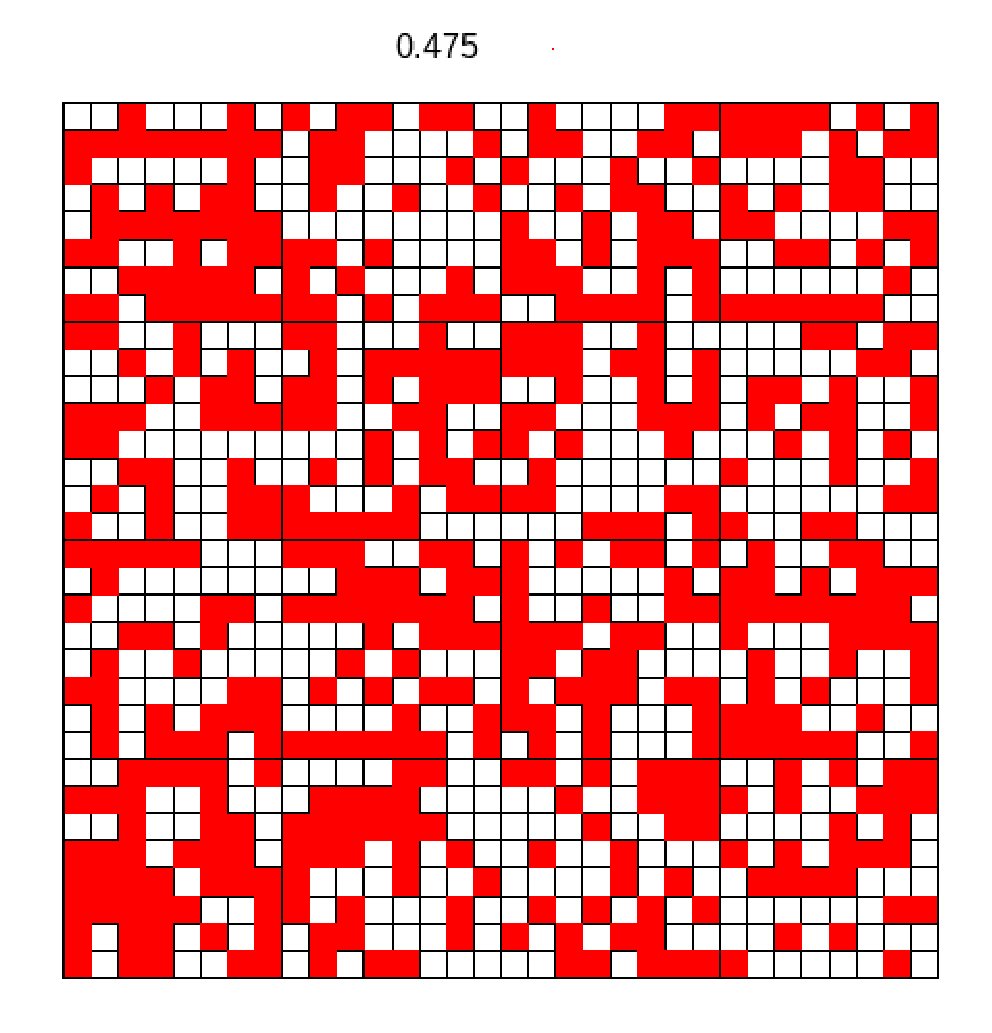
\includegraphics[width=1\linewidth]{L32_1}
\caption{Характерный вид заполненной решетки для $L=32$, в верхней части изображения отображается текущее значение $p$.} %% подпись к рисунку
\label{ris:experimoriginal} %% метка рисунка для ссылки на него
\end{minipage}
\hfill
\begin{minipage}[h!]{0.49\linewidth}
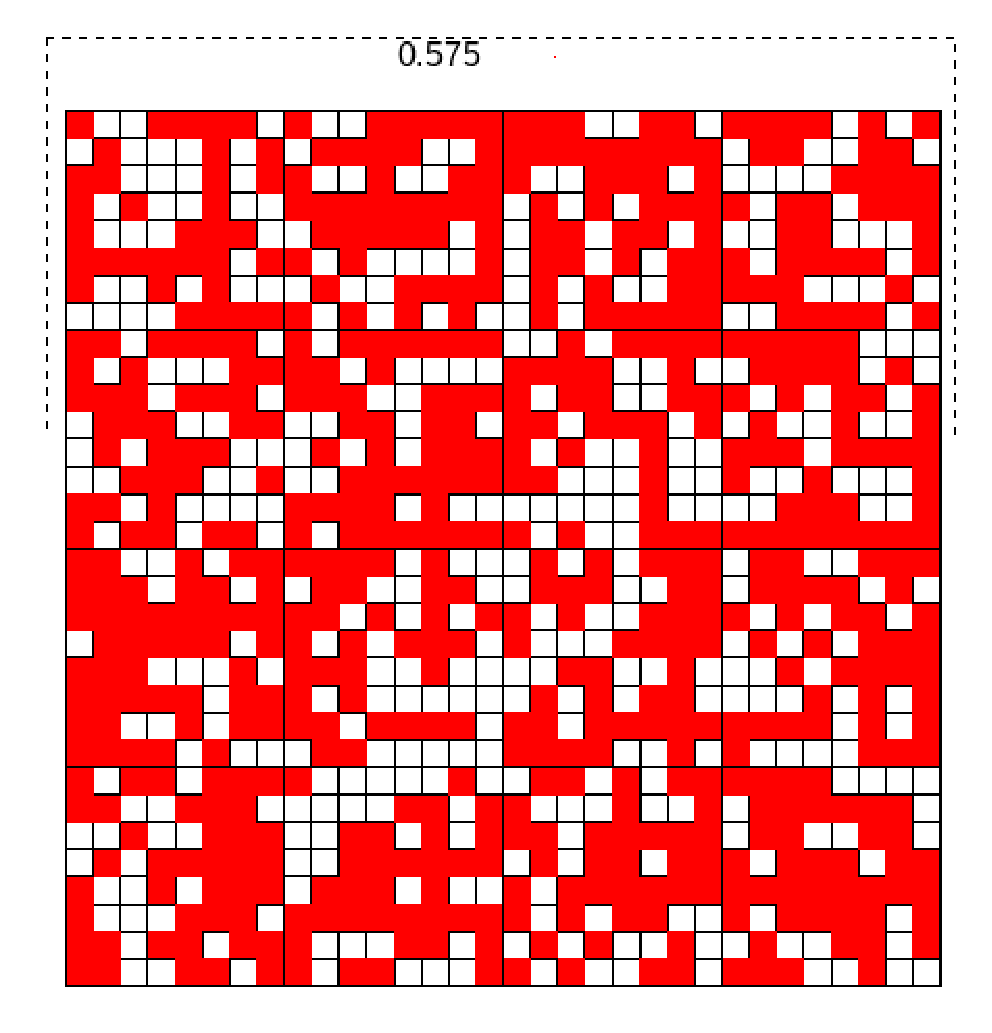
\includegraphics[width=1\linewidth]{L32_2}
\caption{Характерный вид заполненной решетки для $L=32$. В данном случае появился перколяционный кластер.}
\label{ris:experimcoded}
\end{minipage}
\end{center}
\end{figure}

Оценим динамику изменения порога перколяции $p_c$ с увеличением параметра $L$, посчитав среднее значение $p_c$ по $n=10$ испытаниям и среднеквадратичное отклонение этой величины.
\begin{equation}
<p_c>=\frac{1}{n} \sum\limits_{i=1}^n{p_c^i}
\end{equation}

\begin{equation}
\sigma_{p_c}=\frac{1}{n} \sum\limits_{i=1}^n({{p_c}^i-<p_c>})^2
\end{equation}

\begin{table}[h!]
\caption{\label{tab:canonsummary}Значение параметра  $p_c$ для $n=10$ испытаний в случаях c различными значениями $L$.}
\begin{center}
\begin{tabular}{|c|c|c|c|}
\hline
$i$ & $L=4$ & $L=16$ & $L=32$ \\
\hline
1 & 0,375  & 0,550 & 0,575\\
2 & 0,300  & 0,575 & 0,575\\
3 & 0,425  & 0,625 & 0,600\\
4 & 0,400  & 0,625 & 0,600\\
5 & 0,425  & 0,525 & 0,600\\
6 & 0,425  & 0,550 & 0,625\\
7 & 0,400  & 0,625 & 0,600\\
8 & 0,425  & 0,550 & 0,600\\
9 & 0,525  & 0,600 & 0,575\\
10 & 0,275  & 0,550 & 0,625\\
\hline
$<p_c>$ & 0.3975 & 0.5775 & 0.5975 \\
\hline
$\sigma_{p_c}$ & 0,00443125 & 0,00130625 & 0,00030625 \\
\hline
\end{tabular}
\end{center}
\end{table} 



\newpage\section{Выводы}

В ходе данной работы была разработана программа для симуляции ячеечной перколяции при различных размерах квадратной решетки. Был оценен порог перколяции $p_c$ для решетки со стороной $L=4$, $L=16$, $L=32$. Дисперсия порога перколляции с увеличением размеров квадратной решетки при этом уменьшалась. Из n=10 измерений для каждого значения L можно сделать вывод, что при увеличении размеров квадратной решетки точность измерений растет, что характерно для решетки конечного размера.
\end{document}
